AI agents deal with knowledge(data).
\begin{itemize}
\item Facts(believe \& observe knowledge)
\item Procedures("how to" knowledge)
\item Meaning (relate \& define knowledge)
\end{itemize}

Right representation is crucial 
\begin{itemize}
\item Early realisation in AI
\item Wrong choice can lead to project failure
\item Active research area
\end{itemize}

\subsection{Choosing a representation}
For certain problem solving techniques.
\begin{itemize}
\item Best representation already known
\item Often a requirement of the technique
\item Or a requirement of the programming language(e.g. Prolog)
\end{itemize}

Examples:\\
First order theorem proving(first order logic), Inductive logic programming(logic programs) and Neural network learning(neural networks). \\

Some of the general representation schemes are suitable for many different(and new) AI applications. \\

Representation of:
\begin{itemize}
\item Declarative knowledge(what, objects, structure)
\item Procedural knowledge(how, actions, performance)
\end{itemize}

Representation formalisms
\begin{itemize}
\item Declarative knowledge
\begin{itemize}
\item Frames, Semantic Networks, Inheritance Hierarchies, Schemata,...
\end{itemize}
\item Procedural knowledge
\begin{itemize}
\item Algorithms, Procedures, Planes, Rules,...
\end{itemize}
\end{itemize}

\subsubsection{Declarative examples}
Information about items in a store:\\
\begin{lstlisting}
cheaper(coca_cola, pepsi)
tastier(coca_cola, pepsi)

if(cheaper(x, y) && (tastier(x, y))
	then but(x)
\end{lstlisting}

\subsubsection{Procedural example}
Shopping script:
\begin{enumerate}
\item Make a list of all items to buy
\item Walk to the shop
\item For each item on the list, get the item and add it to the shopping
\item Walk to the checkout counter
\item Pack the items
\item Pay
\item Walk home
\end{enumerate}

\section{Aspects of Knowledge representation}
Syntax:
\begin{itemize}
\item Possible (allowed) constructions
\item For example: colour(my\_car, red), my\_car(red), red(my\_car), etc.
\end{itemize}

Semantics:
\begin{itemize}
\item What the representation \textbf{means} (and how it maps to the real world)
\item Example:
\begin{itemize}
\item Colour(my\_car, red) means: "my car is red", "paint my car red", etc.
\end{itemize}
\end{itemize}

Inference:
\begin{itemize}
\item The interpreter
\item Decides what kind of conclusions can be drawn
\item For example: Modus ponens($P, P \rightarrow Q, therefore Q$)
\end{itemize}

\subsection{Well-defined syntax/semantics}
Knowledge representation languages should have precise syntax and semantics.\\
You must know exactly what an expression means in terms of object in the real world.\\
\begin{figure}[h]
\centering
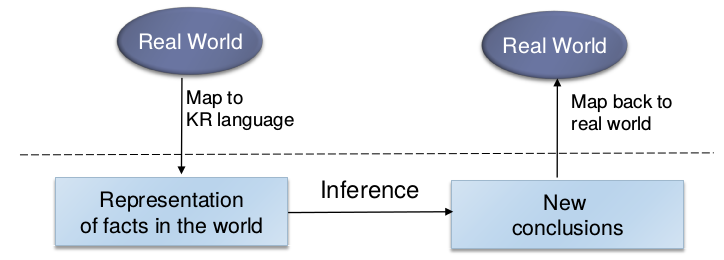
\includegraphics[width=0.6\textwidth]{chap_5Pics/Selection_018.png} 
\caption{Knowledge representation syntax/semantics}
\end{figure}


\subsection{Requirements for Knowledge Representation languages:}
Representation adequacy:
\begin{itemize}
\item Should allow for representing all the required knowledge
\end{itemize}

Infernal adequacy:
\begin{itemize}
\item Should allow the inference of new knowledge
\end{itemize}

Inferential efficiency:
\begin{itemize}
\item Inferring new knowledge should be efficient
\end{itemize}

Clear syntax and semantics:
\begin{itemize}
\item Unambiguous and well-defined
\end{itemize}

Neutralness:
\begin{itemize}
\item Easy to read and use
\end{itemize}

\section{What is a Logic?}
A language with concrete rules.\\
No ambiguity in representation, however there may be errors. Allows for unambiguous communication and processing. \\
Is very unlike natural languages like e.g. English.\\
Many ways to translate between languages\ a statement can be represented in different logics, and possibly differently in same logic. \\

It should not be confused with logical reasoning, logic are languages, reasoning is a process(which may use logic).

\subsection{Non-logical representation}
Logic representation have restrictions and can be hard to work with.
Many AI researches searched for better representations.\\

Non-logical:
\begin{itemize}
\item Semantic networks
\item Conceptual graphs
\item Frames
\item Scripts
\item Production rules
\item ...
\end{itemize} 

\subsection{What we've ignored}
Objects in the world tend to be related to each other.
\begin{itemize}
\item Classes, superclasses \& subclasses, part / whole hierarchies
\item Properties are \textit{inherited} across relationships
\end{itemize}

The state of the world can change over time.
\begin{itemize}
\item Explicit representation of time
\item Frame problem: representing the effects of action in logic without having to represent explicitly a large number of intuitive obvious non-effects
\item Non-monotonic reasoning
\end{itemize}

We must reason without complete knowledge
\begin{itemize}
\item Closed world assumption
\end{itemize}

Not all knowledge is "black \& white":
\begin{itemize}
\item Uncertainty, statistics, fuzzy logic,...
\end{itemize}

Defaults and exceptions:\\
Exception for a single object, a property of the object must be set to the (exception) value.\\

\section{Semantic Networks}
Semantic networks are essentially a generalization of inheritance hierarchies.\\
Each node is an object, class, concept, or event. \\

Each link is a relationship.
\begin{itemize}
\item is-a (the usual sublcass or element relationship
\item has-part or part-of
\item any other relationship that makes sense in context(e.g. owns thing x)
\end{itemize}

Semantic networks represent knowledge as a network or graph(easily stored on the computer). 
By traversing the network we can find:
\begin{itemize}
\item Elephant x likes apples(by inheritance)
\item That certain concepts related in certain ways(e.g. apples and elephants)
\end{itemize}

\section{Frames}
Devised by Marvin Minsky in 1974.\\
Is an extension to semantic networks, and incorporates certain valuable human thinking characteristics:\\
Expectations, assumptions, stereotypes, Exceptions, Fuzzy boundaries between classes.\\

Frames often allowed you to say which things were just typical(*) if a class, and which are definitional, so couldn't be overridden.\\
Frames also allow multiple inheritance(Nellie is an Elephant AND a circus animal).\\

\subsection{Frame representation}






